\documentclass{article}
\usepackage{graphicx}
\usepackage{url}
\usepackage[margin=1.5cm]{geometry}
\usepackage{amsmath}

\begin{document}

\title{Solutions to Homework 2}
\author{Prof. Jordan C. Hanson}

\maketitle

Exercises, Chapter 2: 74, 75a, 76, 78, 79, 80, 83, 84, 88, 92, 93, (94-99)

\begin{enumerate}
\item Exercise 74 (a-b): The 51 and 99 seem to be outliers according to the stem plot (see Tab. \ref{tab:ex74}).
\begin{table}[ht]
\centering
\begin{tabular}{| c | c |}
\hline
\hline
Stem & Leaves \\ \hline
0 &   \\ \hline
1 &   \\ \hline
2 &   \\ \hline
3 &   \\ \hline
4 &   \\ \hline
5 & [1.0] \\ \hline
6 &   \\ \hline
7 & [7.0, 8.0, 6.0, 9.0] \\ \hline
8 & [1.0, 6.0, 2.0, 4.0] \\ \hline
9 & [9.0] \\ \hline
\hline
\end{tabular}
\caption{A stemplot for exercise 74. \label{tab:ex74}.}
\end{table}
\item Exercise 75a:
\begin{figure}[ht]
\centering
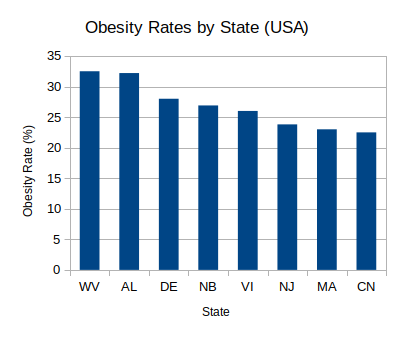
\includegraphics[width=0.3\textwidth]{figures/obesity.png}
\caption{\label{fig:ex75} A bar chart of obesity rates in the USA.}
\end{figure}
\item Exercise 76:
\begin{itemize}
\item a: See Tab. \ref{ex:76a}.
\begin{table}[ht]
\centering
\begin{tabular}{| c | c | c |}
\hline
Books & Freq. & Rel. Freq. \\ \hline
0 & 10 & 0.15 \\
1 & 12 & 0.18 \\
2 & 16 & 0.235 \\
3 & 12 & 0.18 \\
4 & 8 & 0.12 \\
5 & 6 & 0.09 \\
6 & 2 & 0.03 \\
8 & 2 & 0.03 \\
\hline
\end{tabular}
\begin{tabular}{| c | c | c |}
\hline
Books & Freq. & Rel. Freq. \\ \hline
0 & 18 & 0.15 \\
1 & 24 & 0.20 \\
2 & 22 & 0.20 \\
3 & 22 & 0.18 \\
4 & 15 & 0.13 \\
5 & 10 & 0.08 \\
7 & 5 & 0.04 \\
9 & 1 & 0.01 \\
\hline
\end{tabular}
\begin{tabular}{| c | c | c |}
\hline
Books & Freq. & Rel. Freq. \\ \hline
1 & 20 & 0.29 \\
3 & 35 & 0.5 \\
5 & 12 & 0.17 \\
7 & 2 & 0.03 \\
9 & 1 & 0.01 \\
\hline
\end{tabular}
\caption{\label{ex:76a} (Left) Publisher A, (Middle) Publisher B, (Right) Publisher C.}
\end{table}
\item b: See Fig. \ref{fig:ex76b}.
\begin{figure}[ht]
\centering
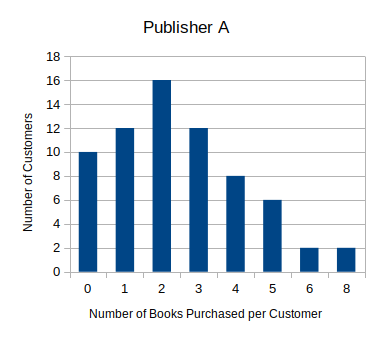
\includegraphics[width=0.3\textwidth]{figures/pubA.png}
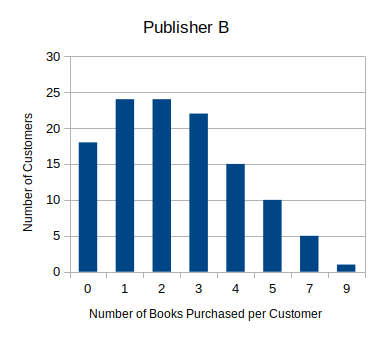
\includegraphics[width=0.3\textwidth]{figures/pubB.png}
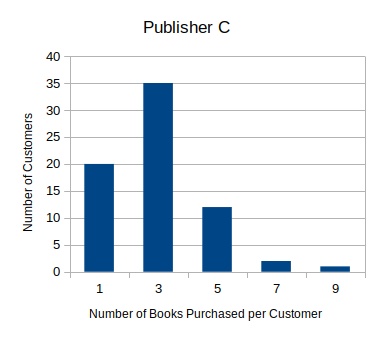
\includegraphics[width=0.3\textwidth]{figures/pubC.png}
\caption{\label{fig:ex76b} Histograms of books purchased by customers of three different companies.}
\end{figure}
\item c: The publisher B data has a different bin design.  The publisher A data and B data have different $N$ values.
\item d: If the people sampled buy books from all three publishers, and the publishers do not specialize in a particular type of fiction paperback, I would expect Fig. \ref{fig:ex76b} (right) to resemble the others.  However, it also has wider bins.
\item e/f: The result is that each plot has the same bin design, and shows the decrease in frequency with increasing number of books purchased.  However, the difference for the 0 and 1 bin varies between publisher A and B.
\end{itemize}
\item Exercise 78: See Fig. \ref{fig:ex78a}. The relative frequencies are 0.2, 0.36, 0.24, 0.16, and 0.04.  The cumulative frequencies are 0.2, 0.56, 0.8, 0.96, and 1.0.
\begin{figure}[hb]
\centering
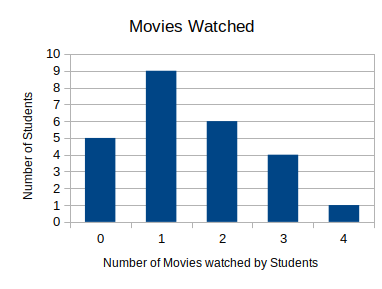
\includegraphics[width=0.35\textwidth]{figures/movies.png}
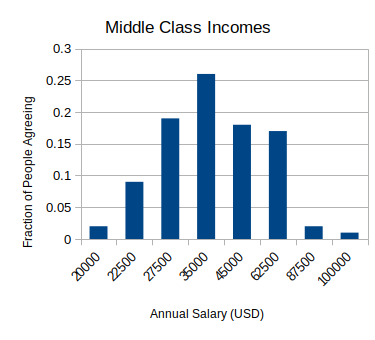
\includegraphics[width=0.3\textwidth]{figures/income.png}
\caption{\label{fig:ex78a} (Left) Movies watched by students. (Right) Annual salaries people associate with the term \textit{middle class}. i) Note the bars do not correspond to constant width.  ii) The smallest and largest bins technically do not have fixed size.}
\end{figure}
\item Exercise 79: (a) 41 percent.
\item Exercise 80: (d) Convenience sampling.
\item Exercise 83: (a) 6 percent (b) 45 percent (c) See Fig. \ref{fig:ex78a} (right). (d) 40th is in the 25,000 - 35,000 bin, and 80th is in the 50,000 to 75,000 bin. (e) See Fig. \ref{fig:ex78a} (right).
\item Exercise 84: (a) Q4, 1.0 (b) Q2, 8.0 (c) Q3 - Q1	 = 10 (d) In the interval 10-13 there is half of the data.  In the other interval there is less than half. (e) ii) does not have 1/4 of the data like the other intervals.
\item Exercise 88: (a) i) Although data 1 has a greater \textit{proportion} above 2 than data 2, we can't know if that's true of the number of total values because the sets could have different $N$ values. ii) Same as (i), we would need to see the individual data points. iii) False: the proportions are equal. (b) Data 2.  Seven is at the far edge of the upper quartile, and farther from the median relative to data 1.
\item Exercise 92: 26.5 percent.
\item Exercise 93: (a) This means the upper two quartiles contain a larger fraction of the data. (b) Life expectance could increase, and people could be having fewer children. (c) No, because it depends on the overall population.
\item Exercise 94-99: 94) 6 years, because half of the data is below 1014. 95) i) 1447.5 ii) 528.5 96) 474 97) 50 percent (Q1 to Q3) 98) 919 FTES, the middle 50 percent of the data. 99) 0.03.
\end{enumerate}

\end{document}
